% Chapter 1

\chapter{Introducción general} % Main chapter title

\label{Chapter1} % For referencing the chapter elsewhere, use \ref{Chapter1} 
\label{IntroGeneral}

En este capítulo se realiza una introducción a la domótica para edificios públicos y monitoreo de oficinas. Asimismo, se explica la motivación, se mencionan algunos sistemas existentes en el mercado, y por último se explica el alcance y objetivos.
%--------------------------------------------------------------------------------------------------------------------------------

% Define some commands to keep the formatting separated from the content 
\newcommand{\keyword}[1]{\textbf{#1}}
\newcommand{\tabhead}[1]{\textbf{#1}}
\newcommand{\code}[1]{\texttt{#1}}
\newcommand{\file}[1]{\texttt{\bfseries#1}}
\newcommand{\option}[1]{\texttt{\itshape#1}}
\newcommand{\grados}{$^{\circ}$}

%--------------------------------------------------------------------------------------------------------------------------------

%\section{Introducción}

%--------------------------------------------------------------------------------------------------------------------------------

\section{Domótica}

Se llama domótica a los sistemas capaces de automatizar una vivienda o edificación de cualquier tipo,y que aporta servicios de gestión energética, seguridad, bienestar y comunicación, y que pueden estar integrados por medio de redes interiores y exteriores de comunicación, cableadas o inalámbricas, y cuyo control goza de cierta ubicuidad, desde dentro y fuera de la edificación. Se podría definir como la integración de tecnología en el diseño inteligente de un recinto cerrado.
El término domótica proviene de la unión de las palabras domus que significa casa en latín y autónomo del griego aftonómos ("que se gobierna a sí mismo").

\subsection{Aspectos principales}

Los servicios que ofrece la domótica se pueden agrupar según cinco ámbitos principales. A continuación, se define y se indican ejemplos de cada uno.

\begin{itemize}
\item Programación y ahorro energético: en muchos casos no es necesario sustituir los aparatos o sistemas del hogar/edificio por otros que consuman menos energía sino realizar una gestión eficiente de los mismos.
\begin{itemize}
\item Climatización y calderas: programación y zonificación, por ejemplo, el uso de un termostato.
\item Encender o apagar sistemas de luz.
\item Con un mando a distancia o control central se puede accionar un producto o agrupación de productos y activar o desactivar el funcionamiento de un sensor.
\item Gestión eléctrica.
\end{itemize}
\item Confort: conlleva todas las actuaciones que se puedan llevar a cabo para mejorar la comodidad de una vivienda o edificio. Dichas actuaciones pueden ser de carácter tanto pasivo como activo.
\begin{itemize}
\item Iluminación: apagado general de todas las luces, automatización del apagado/encendido de cada punto de luz, regulación del nivel de luminosidad.
\item Automatización de los distintos sistemas dotándolos de control eficiente y de fácil manejo.
\item Control vía internet.
\item Generación de programas de forma sencilla para el usuario.
\end{itemize}
\item Seguridad: consiste en una red de seguridad encargada de proteger tanto los bienes patrimoniales, como la seguridad personal y la vida.
\begin{itemize}
\item Alarmas de intrusión: se utilizan para detectar o prevenir la presencia de personas extrañas a una vivienda o edificio.
\item Detectores y alarmas de detección de incendios.
\end{itemize}
\item Comunicaciones: son los sistemas o infraestructuras de comunicaciones que posee el edificio.
\begin{itemize}
\item Transmisión de alarmas.
\item Intercomunicaciones.
\item Control remoto desde internet, PC, mandos inalámbricos (por ejemplo, Wi-Fi).
\end{itemize}
\item Accesibilidad: bajo este mecanismo se incluyen las aplicaciones o instalaciones de control remoto del entorno que favorecen la autonomía personal de personas con limitaciones funcionales, o discapacidad.
\end{itemize}

\subsection{Arquitectura}
\label{sec:arquitecturadedomotica}

Desde el punto de vista de donde reside la inteligencia del sistema domótico, hay varias arquitecturas diferentes:

\begin{itemize}
\item Arquitectura centralizada: un controlador recibe información de múltiples sensores y, una vez procesada, genera las órdenes oportunas para los actuadores.
\item Arquitectura distribuida: toda la inteligencia del sistema está distribuida entre los módulos, sean sensores o actuadores. Suele ser típico de los sistemas cableados o redes inalámbricas.
\item Arquitectura mixta: sistemas con arquitectura descentralizada en cuanto a que disponen de varios pequeños dispositivos capaces de adquirir y procesar la información de múltiples sensores y transmitirlos al resto de dispositivos distribuidos por el edificio.
\end{itemize}

En la figura [\ref{fig:domoticagenerico}] se puede ver el esquema de un sistema de domótica genérico. El componente principal es el controlador, por allí pasa toda la información de los sensores y actuadores, del lado derecho de la figura se muestran ejemplos de actuadores y del lado izquierdo, ejemplos de sensores. La interfaz es muy importante por que es el nexo entre el usuario y el sistema, en la figura se muestra debajo del controlador las interfaces como un teclado, móvil, interruptor o interfaz web.

\begin{figure}[h]
	\centering
	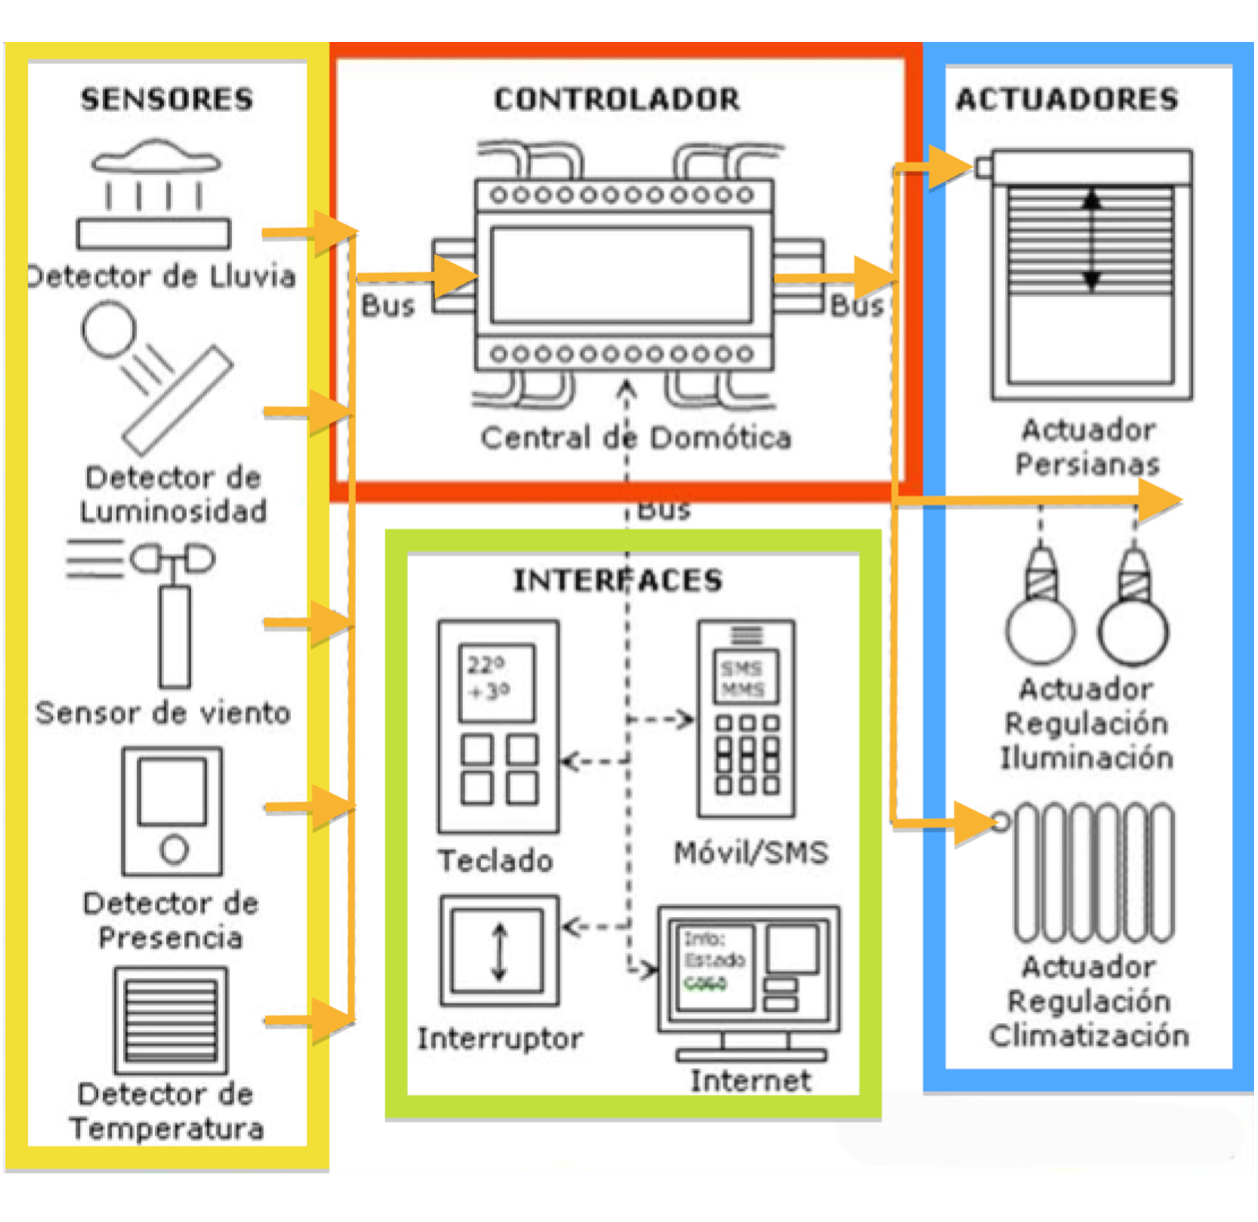
\includegraphics[width=.55\textwidth]{./Figures/domoticagenerico.png}
	\caption{Sistema de domótica genérico.}
	\label{fig:domoticagenerico}
\end{figure}

%--------------------------------------------------------------------------------------------------------------------------------

%\section{Descripción del problema}

%--------------------------------------------------------------------------------------------------------------------------------

\section{Estado del arte}

En la actualidad existe una amplia variedad de sistemas ofrecidos por empresas multinacionales como Fibaro, iHaus, Sonoff, ABB o Schneider Electric, que se encuentran enmarcados dentro de los sistemas de automatización y control de edificios/casas.Estos sistemas fueron tenidos en cuenta para la toma de decisiones en lo referente al desarrollo del trabajo, y por ello se resumen algunas características de estos en la tabla [\ref{tab:sistemasdomotica}].

\begin{table}[h]
	\centering
	\caption[Comparación]{Comparación de equipos en el mercado}
	\begin{tabular}{l c c c}    
		\toprule
		\textbf{Marcas}  	& \textbf{Conectividad}   	&\textbf{Interfaz}  	&\textbf{Monitoreo y Configuración}  						\\
		\midrule
		iHaus				& \ Zigbee 					&\ Display				&\ Software propietario										\\	
		Fibaro				& \ Z-wave					&\ No aplica			&\ WebServer												\\
		Sonoff	 			& \ Wifi/RF 				&\ Display				&\ Software propietario										\\
		ABB		 			& \ KNX 					&\ Display				&\ WebServer												\\
		Schneider E.	 	& \ BACNet 					&\ No aplica			&\ Software propietario										\\
		\bottomrule
		\hline
	\end{tabular}
	\label{tab:sistemasdomotica}
\end{table}

Si bien estos dispositivos se pueden adaptar a edificios de cualquier tipo, uno de los problemas mas usuales en cuanto a las conexiones inalámbricas es el alcance,es decir, la distancia entre el dispositivo central y el nodo. Los dispositivos mas comunes como los de iHaus, Fibaro y Sonoff son efectivos en cuanto al alcance en ámbitos residenciales, es decir, no están preparados para grandes distancias y muros anchos debido a que pierden la conectividad.

Otro aspecto a tener en cuenta en este tipo de dispositivos es la interfaz de usuario. Los sistemas de domótica en la actualidad proponen una gran variedad de opciones para visualizar la información de los sensores y actuadores, pero algunas opciones no terminan siendo aptas para un sistema de gestión en un edificio público y además se debe agregar mas hardware para dicho requerimiento.

En la figura [\ref{fig:ihausesquema}] se puede ver un esquema del sistema de iHaus como representación general de un sistema de domótica comercial \ref{fig:ihausesquema}. Éste cuenta con una central y nodos que funcionan como sensores y actuadores.

\begin{figure}[h]
	\centering
	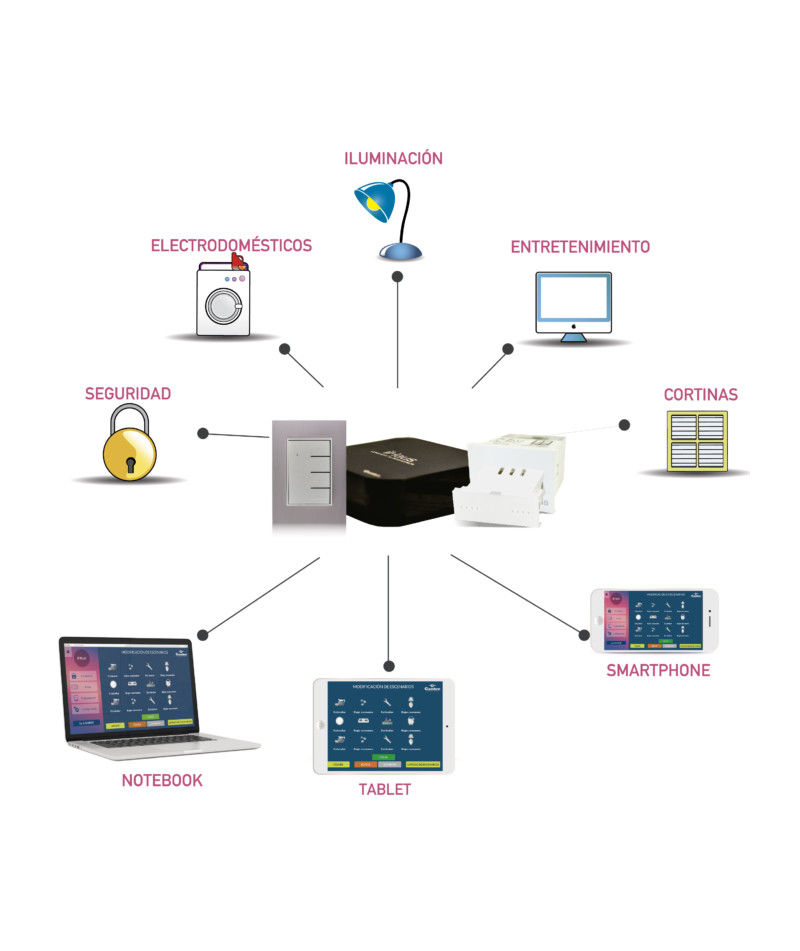
\includegraphics[width=.65\textwidth]{./Figures/ihausesquema.jpg}
	\caption{Sistema comercial de la marca iHaus.}
	\label{fig:ihausesquema}
\end{figure}

%--------------------------------------------------------------------------------------------------------------------------------

\section{Motivación}

%--------------------------------------------------------------------------------------------------------------------------------
Uno de los principales desafíos en la economía actual se refiere a la reducción en el uso de distintos tipos de energías (eléctrica, térmica, etc.) y la huella de CO\textsubscript{2} en los existentes edificios públicos utilizando tecnologías de la información, servicios de monitoreo y manejando el consumo de la energía. Se tiene especial atención a los edificios históricos que son generalmente menos eficientes energéticamente y requieren estrictas restricciones de despliegue para evitar daños por amplia actualización.
Un ámbito muy resignado por los desarrolladores de tecnología son los edificios públicos, debido a la complejidad en la instalación de este tipo de dispositivos. En la Argentina, en el marco del {\textit{Programa de Uso Racional y Eficiente de la Energía (PRONUREE) en Edificios Públicos}}, que tiene como objetivo reducir los niveles de consumo energético de la administración pública nacional mediante:

\begin{itemize}
\item La implementación de medidas de mejora de eficiencia energética.
\item La implementación de criterios para la gestión de la energía.
\item La concientización del personal en el uso racional de la energía.
\end{itemize}

Para cumplir con dicho marco se propone el desarrollo de un kit capaz de generar una red de sensores y actuadores que sean de fácil instalación y además que se pueda extender mediante el uso de la tecnología modular.
Disponer de estos dispositivos en edificios públicos tiene como beneficios:

\begin{itemize}
\item Monitoreo remoto de oficinas, aulas y espacios públicos.
\item Encendido y apagado de luces y aires acondicionados.
\item Mejora de la eficiencia energética de los edificios públicos.
\end{itemize}

En la figura [\ref{fig:esquemaplanteado}] se puede ver un esquema de la propuesta planteada.

\begin{figure}[h]
	\centering
	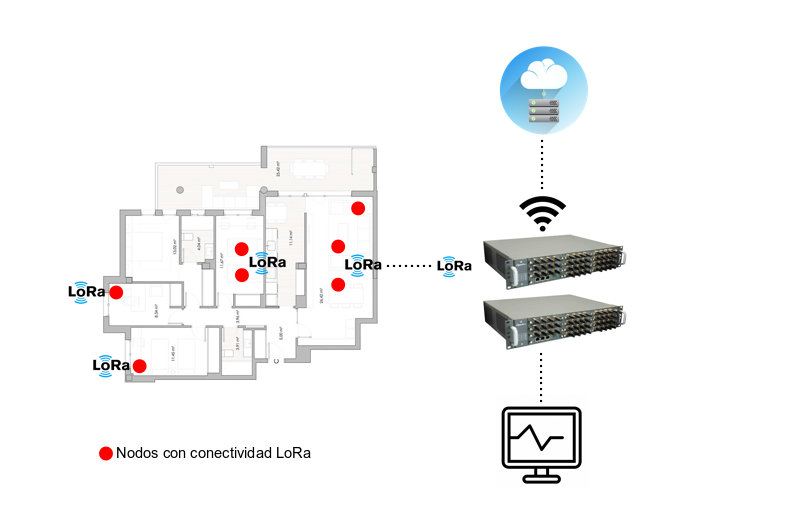
\includegraphics[width=.80\textwidth]{./Figures/esquemaplanteado.png}
	\caption{Esquema del sistema planteado.}
	\label{fig:esquemaplanteado}
\end{figure}


\section{Objetivos y alcances}
\label{sec:FillingFile}

En esta sección se hablará de los objetivos y alcances que tiene este proyecto.

\subsection{Objetivos}

El propósito de este proyecto es desarrollar un prototipo operativo de un sistema de control, monitoreo y supervisión de ciertas funciones y/o parámetros de los edificios, con la capacidad de visualizar la información de interés en un display e informar alertas. Un requisito importante es que su instalación requiera de una intervención mínima. Éste desarrollo permitirá maximizar la eficiencia del edificio, al reducir el consumo de energía y también generar alertas de prevención.

\subsection{Alcance}

Para la realización de este proyecto se desarrollará un primer prototipo operativo del sistema donde se tendrá en cuenta el hardware y software con interfaz de comunicación LoRa ({\textit{Long Range}}). El presente proyecto incluye los siguientes aspectos:

\begin{itemize}
\item Modelado del sistema.
\item Desarrollo del firmware de los nodos y el gateway.
\item Adquisición de datos de una serie de sensores en cada nodo de la red.
\item Transmisión de datos entre los nodos y el gateway mediante el uso del protocolo LoRa a 915 MHz.
\item Uso de base de datos en el gateway para guardar la información de cada nodo.
\item Visualización de los datos adquiridos y parámetros de configuración en una aplicación web.
\item Realización de tests y documentación detallados.
\end{itemize}

%--------------------------------------------------------------------------------------------------------------------------------

%\section{Bibliografía}
%\label{sec:biblio}
%
%Las opciones de formato de la bibliografía se controlan a través del paquete de latex \option{biblatex} que se incluye en la memoria en el archivo memoria.tex.  Estas opciones determinan cómo se generan las citas bibliográficas en el cuerpo del documento y cómo se genera la bibliografía al final de la memoria.
%
%En el preámbulo se puede encontrar el código que incluye el paquete biblatex, que no requiere ninguna modificación del usuario de la plantilla, y que contiene las siguientes opciones:
%
%\begin{lstlisting}
%\usepackage[backend=bibtex,
%	natbib=true, 
%	style=numeric, 
%	sorting=none]
%{biblatex}
%\end{lstlisting}
%
%En el archivo \file{reference.bib} se encuentran las referencias bibliográficas que se pueden citar en el documento.  Para incorporar una nueva cita al documento lo primero es agregarla en este archivo con todos los campos necesario.  Todas las entradas bibliográficas comienzan con $@$ y una palabra que define el formato de la entrada.  Para cada formato existen campos obligatorios que deben completarse. No importa el orden en que las entradas estén definidas en el archivo .bib.  Tampoco es importante el orden en que estén definidos los campos de una entrada bibliográfica. A continuación se muestran algunos ejemplos:
%
%\begin{lstlisting}
%@ARTICLE{ARTICLE:1,
%    AUTHOR="John Doe",
%    TITLE="Title",
%    JOURNAL="Journal",
%    YEAR="2017",
%}
%\end{lstlisting}
%
%
%\begin{lstlisting}
%@BOOK{BOOK:1,
%    AUTHOR="John Doe",
%    TITLE="The Book without Title",
%    PUBLISHER="Dummy Publisher",
%    YEAR="2100",
%}
%\end{lstlisting}
%
%
%\begin{lstlisting}
%@INBOOK{BOOK:2,
%    AUTHOR="John Doe",
%    TITLE="The Book without Title",
%    PUBLISHER="Dummy Publisher",
%    YEAR="2100",
%    PAGES="100-200",
%}
%\end{lstlisting}
%
%
%\begin{lstlisting}
%@MISC{WEBSITE:1,
%    HOWPUBLISHED = "\url{http://example.com}",
%    AUTHOR = "Intel",
%    TITLE = "Example Website",
%    MONTH = "12",
%    YEAR = "1988",
%    URLDATE = {2012-11-26}
%}
%\end{lstlisting}
%
%Se debe notar que los nombres \emph{ARTICLE:1}, \emph{BOOK:1}, \emph{BOOK:2} y \emph{WEBSITE:1} son nombres de fantasía que le sirve al autor del documento para identificar la entrada. En este sentido, se podrían reemplazar por cualquier otro nombre.  Tampoco es necesario poner : seguido de un número, en los ejemplos sólo se incluye como un posible estilo para identificar las entradas.
%
%La entradas se citan en el documento con el comando: 
%
%\begin{verbatim}
%\citep{nombre_de_la_entrada}
%\end{verbatim}
%
%Y cuando se usan, se muestran así: \citep{ARTICLE:1}, \citep{BOOK:1}, \citep{BOOK:2}, \citep{WEBSITE:1}.  Notar cómo se conforma la sección Bibliografía al final del documento. 
